\documentclass[../DISSERTACAO_MAIN.tex]{subfiles}

\begin{document}

Mais de uma década após o advento do sequenciamento de nova geração (NGS, do inglês “Next Generation Sequencing”) \cite{Margulies2005}, é evidente que essa tecnologia incrível e madura promoveu um aumento sem precedentes na geração de dados genômicos e uma importante redução dos custos de sequenciamento \cite{Mardis2008, Goodwin2016}. A fim de reunir e democratizar o acesso a dados genômicos, a International Nucleotide Sequence Database Collaboration (INSDC, http://www.insdc.org/) foi estabelecida em 1987. Esse esforço contínuo compreende três centros internacionais: (i) o National Center for Biotechnology Information (NCBI), (ii) European Bioinformatics Institute (EBI) e (iii) DNA Data Bank of Japan (DDBJ) \cite{Karsch-Mizrachi2018, Cochrane2006}. Como parte dessa notável iniciativa, o banco de dados Sequence Read Archive (SRA) foi criado para hospedar reads e metadados de sequências brutas geradas por projetos NGS \cite{Kodama2012}. Disponibilizar dados brutos de sequenciamento é fundamental para a reprodutibilidade experimental \cite{Stodden2018}, um pilar do esforço científico. Além disso, o SRA tem sido utilizado recorrentemente para apoiar novas pesquisas, tais como: a avaliação de polimorfismos e deleções de base única \cite{Bordbari2017}, o teste de novos programas de bioinformática \cite{Simpson2009, Langmead2012, Bolger2014}, para avaliar os impactos de alguns procedimentos comuns sobre os dados, como o trimming \cite{DelFabbro2013}, dentre outros estudos \cite{Kayal2015, Bernstein2017, Linard2018} .

A disponibilidade de dados públicos está crescendo em conjunto com os potenciais usos de tais bancos de dados para a comunidade científica. Em um período de 2 anos (agosto-2015 a agosto-2017), 3000 trilhões de pares de bases (pb) foram adicionados ao SRA, promovendo um crescimento de 233 \% do repositório  (Karsch-Mizrachi, Takagi \ Cochrane, 2017)\footnote{Essa versão da dissertação foi desenvolvida apenas para experimentar as funcionalidades do \LaTeX{}. Assim sendo, algumas referências que estão no texto -  as que não apresentam hyperlink - não serão encontradas na \autoref{references}. O mesmo é válido para a italização de nomes científicos e termos estrangeiros. Para a versão final dessa dissertação, acesse a cópia presente em meu \href{https://github.com/gavieira/apresentacoes/blob/master/DISSERTA\%C3\%87\%C3\%83O_GABRIEL_ALVES_VIEIRA.pdf}{github} ou a disponível no \href{http://www.bioqmed.ufrj.br/quimica-biologica/dissertacoes-e-teses}{portal  do Departamento de Bioquímica Médica da UFRJ} (ano de defesa: 2019)}. No entanto, o potencial desses dados está longe de ser totalmente explorado, uma vez que os bancos de dados públicos apresentam recursos que poderiam ser usados para abordar diversos tipos de questões biológicas previamente inexploradas. Neste trabalho, nos concentramos em obter genomas mitocondriais completos usando conjuntos de dados (datasets) genômicos disponíveis publicamente.


\section{Bases moleculares do Sequenciamento de Nova Geração Illumina}

Este trabalho se valeu exclusivamente de conjuntos de dados genômicos paired-end gerados pela plataforma Illumina. Segundo o \href{https://www.illumina.com/documents/products/illumina\_sequencing\_introduction.pdf}{site da companhia}, o processo de sequenciamento gerado por essa tecnologia pode ser dividido em 4 etapas principais:

\begin{figure}[htb]
	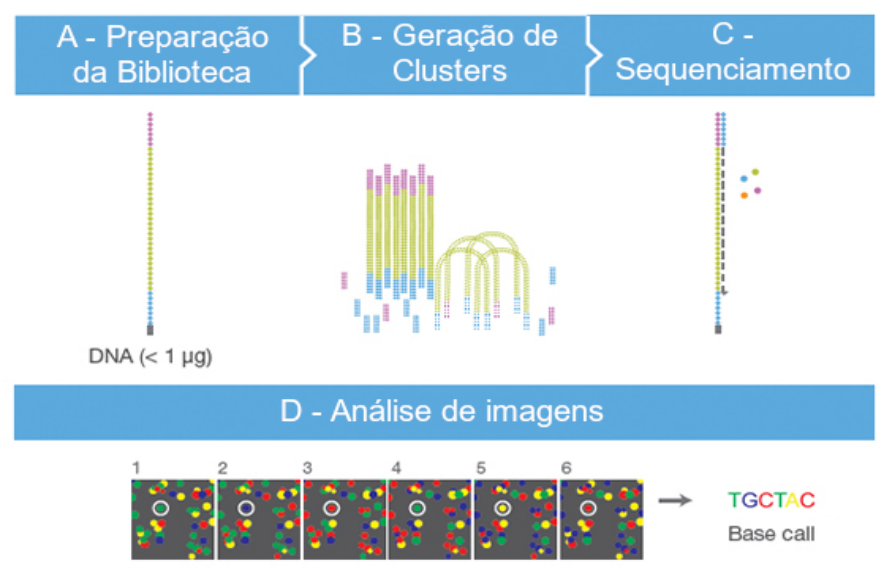
\includegraphics[width=\linewidth]{illumina}
	\caption[Principais etapas do sequenciamento Illumina]{\textbf{Quatro principais etapas do sequenciamento Illumina.}}
	\legend{\textbf{A.} O DNA obtido a partir do organismo de interesse (seja ele DNA genômico ou cDNA, no caso de RNA-Seq) é modificado de forma a gerar uma biblioteca. \textbf{B.} Os fragmentos dessa biblioteca são então ligados à flowcell  e amplificados, gerando aglomerações da mesma sequência (clusters). \textbf{C.} Uma nova sequência é sintetizada pela adição de bases complementares às sequências dos clusters. Cada uma das quatro bases emite um sinal luminoso de coloração específica que é capturado em imagens. \textbf{D.} Essas imagens são analisadas de forma a determinar qual base foi adicionada em cada ciclo de sequenciamento. Adaptado de: \url{https://www.illumina.com/science/technology/next-generation-sequencing/sequencing-technology/2-channel-sbs.html}}
	\label{fig_illumina}
\end{figure}


\textbf{Preparação de biblioteca (\autoref{fig_illumina}-A):} O DNA do organismo de interesse deve ser clivado aleatoriamente (por processos como sonicação ou uso de nucleases inespecíficas) (Knierim et al., 2011). Após isso, fragmentos são selecionados por tamanho através de gel, se obtendo assim sequências com menor variação de tamanho. A preparação das bibliotecas consiste na modificação e amplificação desses fragmentos para que o sequenciamento seja possível. Em um primeiro passo, oligonucleotídeos específicos (chamados adaptadores) se ligam às duas extremidades do fragmento. Na preparação de uma biblioteca, geralmente são usados dois adaptadores: uma para cada extremidade do fragmento (5’ e 3’). A sequência dos adaptadores varia de acordo com o modelo de sequenciador utilizado e contêm tanto regiões de ligação a primers, quanto sequências identificadoras (índices) e uma região imobilizadora, que consiste de oligonucleotídeos necessários para a ligação da sequência à flowcell (mais informações na próxima etapa). O tamanho da sequência proveniente do organismo, a qual se encontra entre os adaptadores, é chamado de insert size. Depois da adição dos adaptadores, os fragmentos podem ser amplificados pela Reação em Cadeia da Polimerase (PCR, do inglês “Polymerase Chain Reaction”). Essa etapa de amplificação (também chamada de “enriquecimento de biblioteca”) nem sempre é realizada, mas é importante por tornar possível a realização de sequenciamentos mesmo a partir de baixas concentrações de DNA. 

\textbf{Ligação e amplificação dos fragmentos na flowcell (\autoref{fig_illumina}-B):}  A biblioteca gerada é então dispersa pela flowcell, que consiste em uma placa de vidro com um número definido de canais (lanes) densamente populados com oligonucleotídeos. Os adaptadores apresentam sequências que são complementares àquelas presentes nesses canais, hibridizando-se a elas e fixando à flowcell  os fragmentos de DNA que serão sequenciados. Essa hibridização se dá de forma aleatória e ocorre com apenas uma das extremidades do fragmento de DNA original, de forma que, em um cenário ideal, é esperado que as sequências se liguem e fiquem posicionadas a uma distância considerável uma das outras, muito embora isso dependa de outros fatores, como a concentração da biblioteca. 

Como a próxima etapa do sequenciamento depende da captação de sinal luminoso, há a necessidade de que cada sequência da flowcell gere cópias que estejam próximas a ela para a amplificação desse sinal. Primeiramente, são adicionadas polimerases que gerarão o reverso complementar das sequências de DNA originais. Então, a fita original é lavada e permanecem apenas seus complementares na placa, que passam pelo processo de “amplificação em ponte” (Mayer et al., 2011). Nesse processo, o adaptador do topo do fragmento se hibridiza a uma sequência complementar na superfície da flowcell. Isso fornece uma extremidade livre que permite a amplificação de uma nova cópia de DNA, a princípio resultando em uma dupla fita que é posteriormente desnaturada e dá origem a duas sequências complementares. Em um novo ciclo, os adaptadores dessas sequências novamente se hibridizam aleatoriamente com aqueles presentes na placa, gerando de forma clonal outras sequências.  Repetido múltiplas vezes, esse processo acaba por amplificar várias cópias de um fragmento a ser sequenciado, que ficam próximos e consequentemente emitem um sinal luminoso mais forte, perceptível pelo sequenciador. A essas aglomerações de cópias de uma mesma sequência se dá o nome de cluster. 

A princípio, os fragmentos em questão podem ser tanto da sequência senso (forward) quanto da antissenso (reverse). Entretanto, para evitar a captação de sinais luminosos conflitantes na próxima etapa, cada etapa de sequenciamento deve ser feita exclusivamente com sequências senso ou antissenso. Isso proporciona dois tipos principais de sequenciamento: (i) single-end, no qual as sequências antissenso são removidas e apenas as sequências senso são sequenciadas; e (ii) paired-end, onde após o sequenciamento das sequências senso, ocorre uma nova série de amplificações em ponte e o processo inverso é realizado, removendo os fragmentos forward e mantendo os reverse. Com isso, ambas as fitas são sequenciadas e, consequentemente, as duas extremidades do fragmento. Conhecendo as extremidades da sequência e o tamanho dos fragmentos gerados, podemos estimar a distância entre as reads. A obtenção dessa informação é a maior vantagem do sequenciamento paired sobre o single-end, já que saber a distância entre sequências nos permite, dentre outros, fechar gaps reais e estabelecer a ordem e distância entre dois ou mais contigs durante a montagem. O uso dessa informação nas montagens frequentemente aumenta o tamanho dos contigs/scaffolds obtidos e consequentemente gera uma representação mais fidedigna do genoma estudado.

Em trabalhos de sequenciamento de genoma nuclear é comum se usar dados advindos de bibliotecas de diferentes tamanhos médios para se obter uma montagem de maior qualidade \cite{Rubin2016, Wirthlin2018}. Vale ressaltar que o tamanho de fragmento ou insert size aceito pelo sequenciamento paired-end é limitado (200-800 pb) e para se conseguir ordenar e unir contigs muito afastados geralmente se faz necessário o uso de um terceiro tipo de sequenciamento: o mate-pair, que consegue obter sequências separadas por uma distância muito maior (2000-5000 pb). A única diferença do sequenciamento mate-pair para o paired-end está na preparação de sua biblioteca (\autoref{fig_biblioteca}): enquanto o paired-end usa os fragmentos gerados na fragmentação diretamente na preparação da biblioteca, no sequenciamento mate-pair moléculas de biotina são ligadas covalentemente às extremidades de DNA (biotinilação), o que leva à circularização dos fragmentos. Posteriormente, os fragmentos são clivados na região de circularização, que é então enriquecida. Assim, as extremidades sequenciadas correspondem às sequências que estão separadas por distâncias muito maiores do que aquelas encontradas em paired-end.

\begin{figure}[htb]
	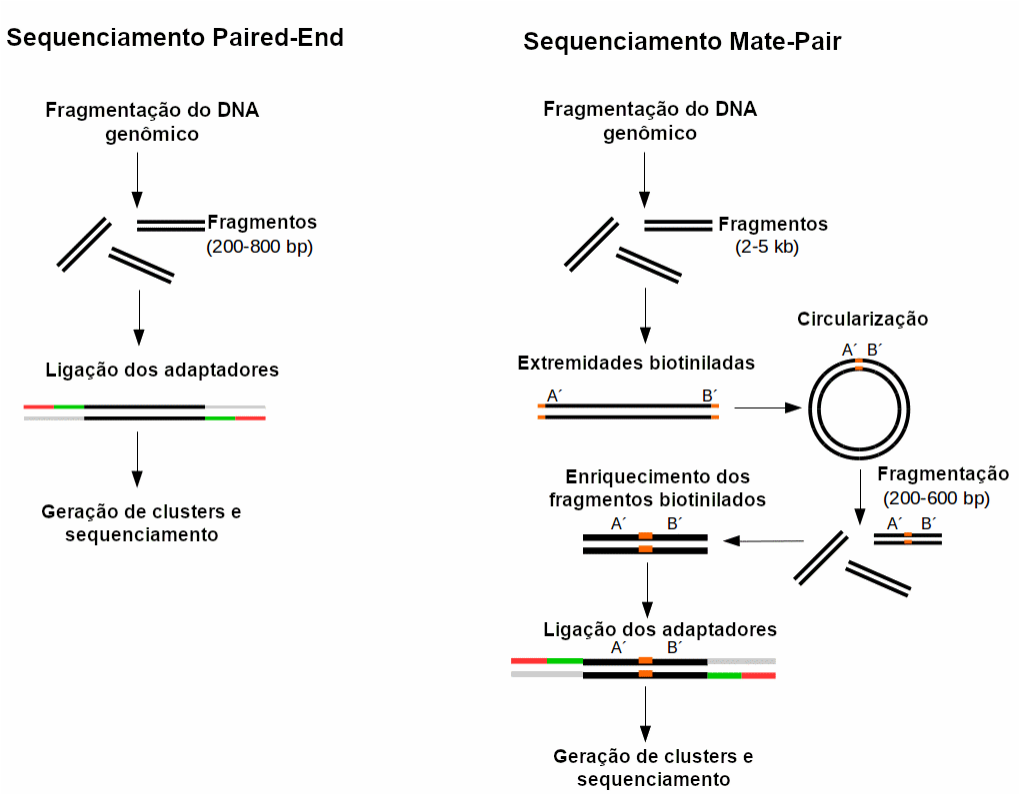
\includegraphics[width=\linewidth]{biblioteca}
	\caption[Preparação de bibliotecas \textit{paired-end} and \textit{mate-pair}]{\textbf{Comparação entre o processo de preparação de bibliotecas \textit{paired-end} e \textit{mate-pair}}}
	\legend{Adaptado de: \url{https://www.ecseq.com/support/ngs/what-is-mate-pair-sequencing-useful-for}}
	\label{fig_biblioteca}
\end{figure}

\textbf{Sequenciamento (\autoref{fig_illumina}-C)}: O processo é baseado no “Sequenciamento por Síntese” (Sequencing-by-Synthesis ou SBS) (Mardis et al. 2008), metodologia na qual um primer se liga ao adaptador da extremidade livre na flowcell e uma DNA polimerase sintetiza uma nova fita pela incorporação de nucleotídeos marcados com fluorescência. Os quatro tipos de nucleotídeos (A, G, C, T) são adicionados à flowcell simultaneamente e cada um apresenta fluoróforos que emitem um sinal luminoso de comprimento de onda específico. Em outras palavras, cada nucleotídeo emite luz de uma coloração característica, que é registrada pelo sequenciador e usada posteriormente na identificação da base incorporada. Esses nucleotídeos também são bloqueados de forma reversível em sua extremidade 3’OH, o que permite que apenas um nucleotídeo seja adicionado e identificado por ciclo de síntese. Essa incorporação de um único nucleotídeo por ciclo é necessária para, por exemplo, a determinação correta do comprimento de regiões homopoliméricas. 

Após a captação do sinal luminoso, o bloqueador 3’OH é clivado e um novo nucleotídeo é incorporado. Esse processo ocorre simultaneamente para milhões ou mesmo bilhões de clusters e se repete “n” vezes até gerar uma read de tamanho “n” por cluster (esse valor pode ir de 50 a 300, dependendo do sequenciador utilizado). A paralelização massiva dessa metodologia, apesar de gerar reads consideravelmente curtas, permite a geração de uma grande quantidade de dados por corrida de sequenciamento. Isso implica uma diminuição do custo de sequenciamento por nucletoídeo quando comparada à tecnologia de sequenciamento Sanger (Mardis, 2008; van Dijk et al., 2014; Goodwin, McPherson  McCombie, 2016).

\textbf{Análise de imagens (\autoref{fig_illumina}-D)}: Cada vez que uma base é adicionada durante o sequenciamento, o sequenciador captura imagens com as fluorescências emitidas por uma grande quantidade de clusters. Essas imagens serão analisadas pelo software do sequenciador, que identifica a posição dos sinais luminosos emitidos por meio de coordenadas X e Y das imagens. As posições emissoras de fluorescência (correspondentes aos clusters) são chamadas de spots. O software do sequenciador analisa essa imagem e, ao avaliar o comprimento de onda e a intensidade do sinal luminoso obtido, realiza a identificação da base (base call) para cada nucleotídeo adicionado a um determinado spot. Ao final desse processo obtemos as sequências de DNA com base na leitura dessas imagens, que por conta disso são chamadas de reads ou leituras. Em sequenciamentos paired-end, as duas extremidades de um mesmo fragmento de DNA pertencerão a um mesmo spot.

O algoritmo utilizado pode apresentar maior ou menor grau de confiança em sua identificação, que é convertido em um valor de qualidade associado a cada base. Essa informação é relevante em diversos procedimentos. Por exemplo, regiões de baixa confiabilidade podem ser identificadas e removidas para que etapas subsequentes (como a montagem) sejam realizada apenas com o “gold standard” dos dados gerados, diminuindo a presença de ruído nas análises e consequentemente propiciando resultados com maior suporte.


\section{O formato sra e o conceito de ``spot''}

O Sequence Read Archive disponibiliza seus dados primariamente nos formatos fastq e sra. Os arquivos sra geralmente precisam passar por uma conversão para fastq para serem usados na maior parte dos programas de bioinformática. O programa mais comumente utilizado nessa conversão é o fastq-dump, parte do pacote de programas SRAtoolkit, distribuído pelo NCBI. Os arquivos sra apresentam duas grandes vantagens sobre os fastq para trabalhos em larga escala: i) ocupam consideravelmente menos espaço do disco rígido, sendo mais eficientes para o armazenamento de cópias locais, especialmente em se tratando de datasets massivos; e ii) o principal programa utilizado para a conversão de sra para fastq (fastq-dump) permite a manipulação de  diversos parâmetros para gerar arquivos fastq modificados sem a necessidade de os baixar novamente. Várias opções podem ser utilizadas para se obter exatamente o tipo de dado desejado: tamanho mínimo das reads (-M), qualidade das reads (-R), remoção de sequencias adaptadoras (-W), formatação do cabeçalho das reads (--readids e –defline-seq, importantes para que o fastq  seja compatível com alguns programas), dentre outros.

Os arquivos sra são divididos em spots, não em reads. Além disso, há tanto uma opção do fastq-dump para imprimir um número fixo de spots (-X) quanto um que permite separar esses spots e armazenar as reads resultantes em um único arquivo (--split-spot) ou em dois arquivos diferentes (--split-files). Embora as documentações oficiais do NCBI não deixem explícito o que é um spot para esses arquivos, a associação com o conceito introduzido no sequenciamento Illumina é muito provável (https://www.biostars.org/p/12047/). Conforme supracitado, em um spot são sequenciadas tanto a read forward quanto a reverse relativas às extremidades de um fragmento de DNA. Assim sendo, o mais provável é que o conceito de “spot” em um arquivo sra paired-end  seja próximo de algo como “toda a informação gerada por um spot em um sequenciamento”, o que corresponde a dizer que um spot é uma concatenação das reads forward e reverse. Isso é corroborado pelo fato de que, ao se separar os spots, o tamanho das sequências geradas caem pela metade e apresentam os característicos cabeçalhos terminando em “1” ou “2” para indicar os pares de sequencias advindas do mesmo fragmento. O dataset paired-end SRR5852657, para o qual mitocôndrias de camundongo (Mus musculus) foram isoladas e sequenciadas (https://www.ncbi.nlm.nih.gov/sra/?term=SRR5852657), foi utilizado na avaliação da diferença observada entre reads geradas com relação à separação de spots (\autoref{fig_spots}). Esse mesmo dataset foi utilizado para gerar arquivos fastq e montar o genoma mitocondrial do camundongo usando uma referência da mesma espécie (KY018919.1). A anotação dos mitogenomas obtidos com e sem a separação de spots da \autoref{fig_anotacao} evidencia que o uso de spots não partidos acarreta mais erros de montagem. 

As sequências concatenadas em um spot, por não corresponderem àquelas encontradas no organismo de estudo, não são recomendadas para realizar montagens. Com isso, concluímos que entender o conceito de spots e utilizar a opção “split-spot” ou “split-files” do fastq-dump é fundamental para se trabalhar com dados públicos resultantes de sequenciamento paired-end.

\section{Montagem e anotação de genomas}

Como o sequenciamento gera sequências curtas, a montagem dessas reads é necessária para se obter sequências maiores ou mesmo genomas completos. O processo de montagem consiste na junção de reads contíguas guiada pela sobreposição dos nucleotídeos presentes em suas extremidades, o que permite gerar sequências maiores (chamadas de contigs). Também há os scaffolds, que consistem em contigs adjacentes cujo afastamento consegue ser estimada pela distância entre as reads geradas por sequênciamentos paired-end ou mate-pair. Como as bases que ligam os contigs não são conhecidas, elas são substituídas por “N”s, que podem ser lidos como “bases desconhecidas” (\autopageref{fig_pairedend}).

\begin{landscape}

\begin{figure}[htb]
		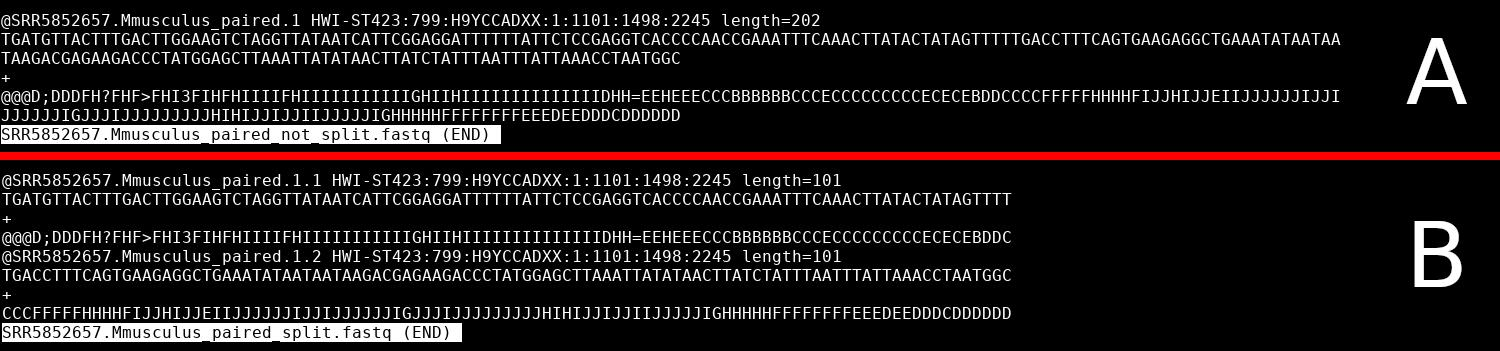
\includegraphics[width=\linewidth]{spots}
		\caption[Conversão de um único spot do formato sra para fastq]{\textbf{Conversão de um único spot do formato sra para fastq usando o software fastq-dump}}
		\legend{O dataset mitocondrial SRR5852657 foi utilizado para se obter um único spot com cabeçalho adaptado para dados paired-end (opções “-X 1” e “--read-ids”). Em \textbf{A}, nenhuma outra opção foi especificada, e o spot corresponde a uma única sequência de 202 nucleotídeos, que corresponde à concatenação das duas reads de 101 pb geradas em \textbf{B} (onde a opção “--split-spot” foi utilizada). As reads de \textbf{B} também se diferenciam pelo cabeçalho (.1 e .2), indicando que elas vieram do mesmo fragmento sequenciado, ao contrário de \textbf{A}.}
		\label{fig_spots}
\end{figure}

\begin{figure}[htb]
	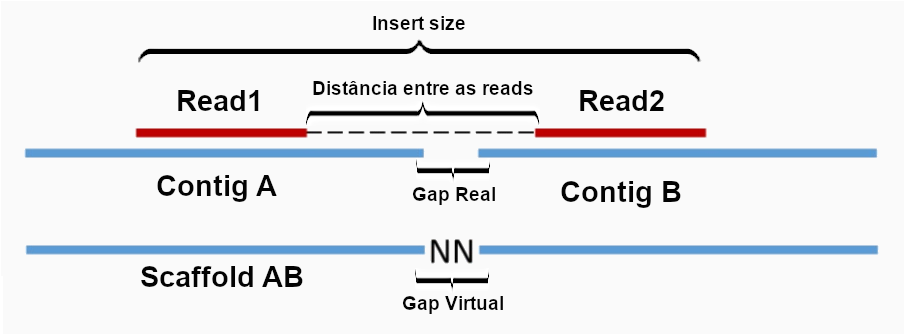
\includegraphics[width=\linewidth]{pairedend}
	\caption[Uso de dados pareados para o fechamento de gaps]{\textbf{Uso de dados pareados para o fechamento de gaps} }
	\legend{Em dados pareados (paired-end ou mate-pair) é possível estimar a distância entre as reads, já que tanto o tamanho do fragmento sequenciado (Insert size) quanto o das sequência em si são conhecidas. Logo, quando as reads pareadas são mapeadas em contigs diferentes, podemos calcular a distância entre eles e uní-los em uma única sequência (scaffold). No processo de fusão, o que antes era um gap real (no qual tanto o tamanho quanto a sequência entre os contigs é desconhecida) se torna um gap virtual (onde se conhece a extensão do gap, que é preenchida por N’s). Adaptado de: http://madsalbertsen.github.io/multi-metagenome/docs/step10.html}
	\label{fig_pairedend}
\end{figure}

\end{landscape}
\documentclass[../DISSERTACAO_MAIN.tex]{subfiles}
\begin{figure}[htb]
	\includegraphics[width=\linewidth]{anotacao}
	\caption[Anotação de montagens mitocondriais e separação de spots] {\textbf{Anotação de montagens mitocondriais com e sem a separação de spots}}
	\legend{Por meio do software MIRA (Chevreux et al., 1999), realizamos montagens mitocondriais por referência para averiguar o impacto das separação dos spots nas montagens. A referência utilizada e os mitogenomas gerados foram anotados utilizando o  MITOS Web Server \cite{Bernt2013}. Podemos observar que a montagem \textbf{A} (obtida através do Genbank – Acession number \href{https://www.ncbi.nlm.nih.gov/nuccore/KY018919.1}{KY018919.1}) não apresenta nenhum problema em sua anotação. As duas outras montagens foram realizadas utilizando a sequência de \textbf{A} como backbone. Na montagem \textbf{B} (obtida usando spots partidos), o tRNA da fenilalanina (trn-F) não pôde ser identificado. Por último, temos que a anotação da montagem \textbf{C} (spots inteiros) apresenta mais problemas: além da ausência de trn-D e trn-F, há vários genes duplicados. De maneira geral, a anotação de \textbf{B} é muito mais similar à da referência, o que sugere que a separação de spots é importante para a obtenção de sequências de maior qualidade.}
	\label{fig_anotacao}
\end{figure}

%\newpage

Há dois tipos principais de montagem (Lesk, 2014): 

\begin{enumerate}[label=(\roman*)]
		\item a montagem de novo, na qual somente a informação de sobreposição/distância entre as reads é utilizada na montagem de uma sequência (chamada de sequência consenso~-~\autoref{fig_montagem}-A)
	\item  a montagem por referência, na qual informação exterior (na forma de uma sequência já existente, chamada de referência ou backbone) é utilizada na montagem. As reads são mapeadas a essa referência que idealmente deve pertencer a um organismo evolutivamente próximo do objeto de estudo, e a sobreposição entre as sequências é então utilizada para se obter o consenso (\autoref{fig_montagem}-B).
\end{enumerate}

 Entretanto, geralmente priorizamos realizar montagens de novo pois elas não incluem viéses associados  a referências, que levam a erros de montagem quando, por exemplo, a referência apresenta ordem gênica (sintenia) diferente daquela encontrada no genoma que está sendo montado. Além disso, ao se trabalhar com organismos não-modelo, referências próximas ao objeto de estudo comumente não estão disponíveis.

Múltiplos algoritmos foram desenvolvidos para a montagem de genomas, mas os mais amplamente utilizados são aqueles que se baseiam nos Grafos de Bruijn (Compeau et al., 2011; Lesk, 2014). Nas implementações desse algoritmo, uma subsequências das reads de tamanho k (chamadas de k-mers) são os vértices e arestas direcionadas são traçadas entre os k-mers nos quais há uma sobreposição de k-1 nucleotídeos, visitando cada nó apenas uma vez (\autoref{fig_brujin}). Ao ser resolvido, o grafo nos dá um caminho entre os nós que indica a sucessão de sequências contíguas sobrepostas, correspondente à sequência montada. O valor de k-mer é geralmente estabelecido por aquele que irá montar o genoma, e a escolha do k-mer mais adequado é pautado pelo balanço entre especificidade e sensibilidade. Por exemplo, ao se escolher k-mers longos, se torna mais fácil estabelecer a direção correta do grafo em uma região repetitiva de DNA ou na ocorrência de erros de sequenciamento (alta especificidade), mas o número de reads sobrepostas acaba sendo muito reduzido (baixa sensibilidade), o que pode levar a uma montagem muito fragmentada. Por outro lado, k-mers curtos geralmente não conseguem resolver corretamente regiões repetitivas do genoma, mas conseguem recrutar um número consideravelmente maior de reads para a montagem.

\begin{figure}
	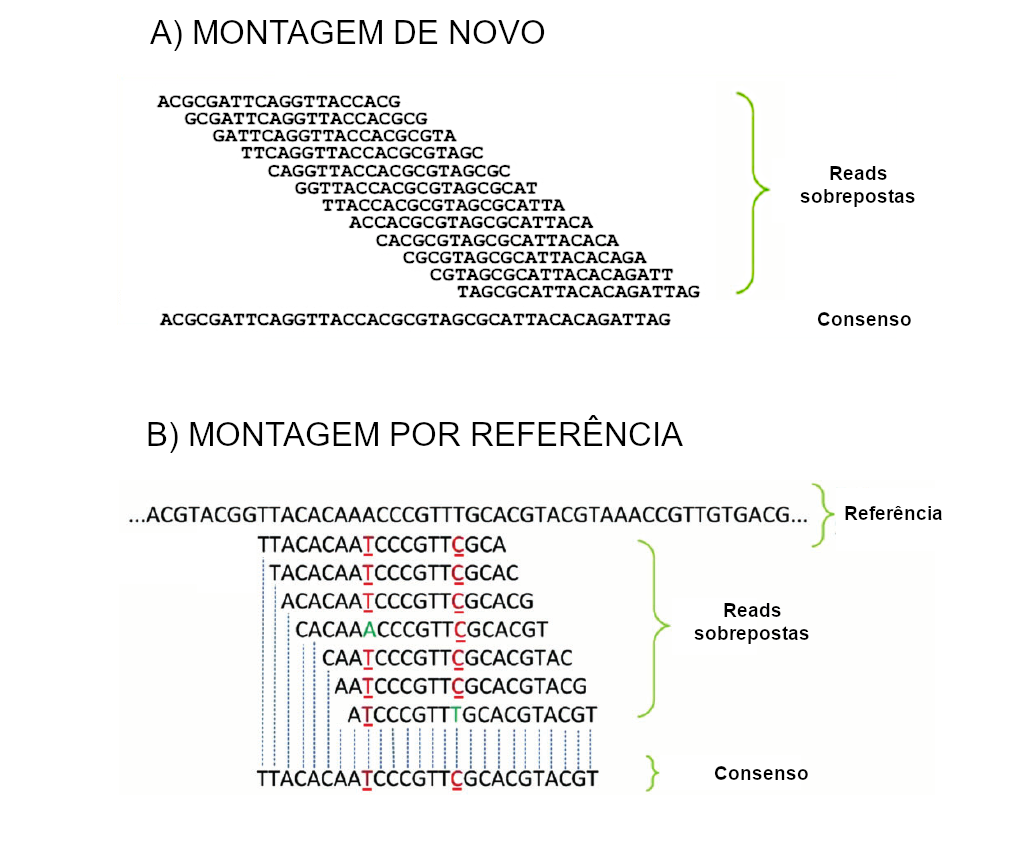
\includegraphics[width=\linewidth]{montagem}
	\caption[Esquema representativo das montagens denovo e por referência]{\textbf{Esquema representativo das montagens denovo e por referência}}
	\legend{\textbf{A.} A montagem de novo se vale exclusivamente da informação contida no sequenciamento. Adaptado de \url{https://contig.files.wordpress.com/2010/02/alignment1.jpg}. \textbf{B.} A montagem por referência utiliza informação externa na forma de uma sequência previamente sequenciada. Adaptado de Wajid  Serpedin (2014). Ambas geram a sequência final com base no consenso das sobreposições.} 
	\label{fig_montagem}
\end{figure}

\begin{figure}
	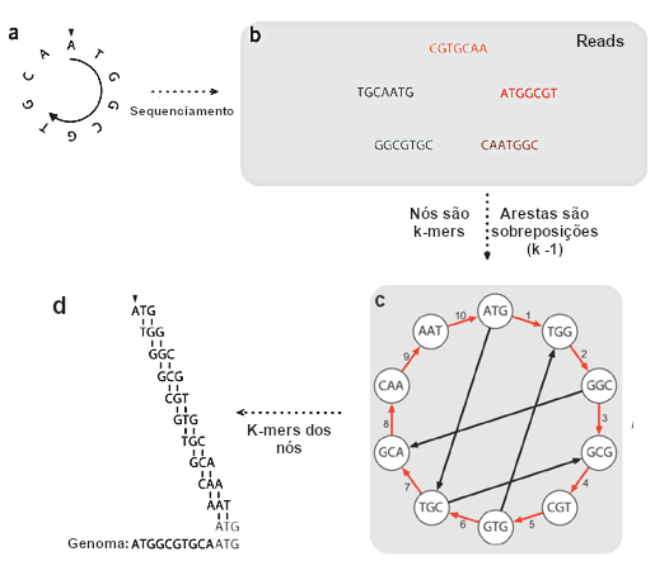
\includegraphics[width=\linewidth]{brujin}
	\caption[Grafos de Bruijn aplicados à montagem de genomas]{\textbf{Grafos de Bruijn aplicados à montagem de genomas}}
	\legend{ \textbf{A}. Um pequeno genomas circular é sequenciado. \textbf{B}. As reads são geradas (cada uma com sete nucleotídeos). \textbf{C}. Com k=3, um grafo de Bruijn é construído, onde os nós são sequências de três nucleotídeos (3-mers) e as arestas são traçadas ao se encontrar sobreposições de dois (k-1) nucleotídeos entre as sequências. Repare que o baixo valor de k-mer utilizado facilita a sobreposição entre vários nós, o que faz com que múltiplos caminhos sejam possíveis nesse grafo (arestas pretas) e dificultam a montagem. \textbf{D}. Ao final, o caminho que visita cada nó apenas uma vez (arestas vermelhas) nos dá a sequência montada. Adaptado de Compeau et al. (2011).}
	\label{fig_brujin}
\end{figure}


Múltiplas sequências podem se sobrepor em uma mesma região, e o número de reads que se sobrepõem confirmando uma determinada base é denominado cobertura (Verli, 2014). Esse conceito pode ser estendido para o cálculo da cobertura média do genoma inteiro que consiste na divisão do total de bases sobrepostas (ou seja, número de reads multiplicado pelo tamanho das mesmas) pelo total de bases da montagem. De forma geral, a cobertura está associada à qualidade da montagem, já que regiões de baixa cobertura apresentam menos dados confirmando sua sequência e consequentemente estão mais sujeitas a estarem incorretas.

A montagem, por melhor que seja, contempla apenas a sequência de nucleotídeos encontrada no objeto de estudo, o que geralmente é insuficiente. Para complementar essa informação e realizar análises adicionais que revelem novos aspectos sobre a biologia do organismo estudado, elementos relevantes dessa sequência nucleotídica (como genes codificadores de proteínas, tRNAs, rRNAs e afins) devem ser identificados e nomeados na montagem. A esse processo de adição de informação funcional às sequências montadas se dá o nome de anotação (Verli, 2014), a qual geralmente é feita em duas etapas: primeiramente, é realizada a anotação automática, que se vale de programas que, geralmente por meio do alinhamento de sequências contra bancos de dados de genes conhecidos (Wyman et al., 2004; Bernt et al., 2013), identificam a localização de vários ou mesmo de todos os genes presentes na sequência fornecida. Entretanto, muitas vezes o estabelecimento dos limites gênicos não é tão preciso, fazendo-se necessária uma segunda etapa de curadoria manual para confirmar ou refinar os resultados obtidos pela anotação automática.

\section{Mitogenomas: evolução, aplicações e ubiquidade em datasets}

Em animais, a mitocôndria é uma organela de origem materna  - salvo raras exceções, como em algumas espécies de bivalves (Zouros et al., 1994; Theologidis et al., 2008) - na qual ocorre o processo de fosforilação oxidativa, indispensável para a obtenção primária de energia em eucariotos. Essa organela está envolvida não só no metabolismo energético \cite{Brand1997}, como também na apoptose (Wang, 2001), diferenciação celular \cite{Wanet2015} e várias doenças \cite{Chan2006}. Apesar da gênese dessa organela ser tópico de discussão ainda hoje, classicamente sua origem comumente é explicada por meio da teoria endossimbiótica, a qual dita que a mitocôndria evoluiu a partir de uma bactéria de vida livre fagocitada e incorporada por uma célula hospedeira \cite{Gray2017}. Algumas características mitocondriais corroboram essa hipótese, como a presença de dupla membrana e ribossomos similares aos encontrados em procariotos, mas nenhuma delas é tão contundente quanto a presença de DNA nessas organelas \cite{Gray1999, Kutschera2005} . O genoma mitocondrial (também chamado de mitogenoma) também apresenta similaridades com um genoma procarioto típico: possui arranjo circular e, no caso do mitogenoma animal, cada fita é transcrita como um único mRNA policistrônico que é então clivado, dando origem a todos os elementos funcionais desse mitogenoma \cite{Boore1999}.

O conteúdo gênico mitocondrial varia consideravelmente em diferentes linhagens de eucariotos, o que acredita-se ocorrer em grande parte devido à transferência de vários genes mitocondriais para o núcleo durante a evolução da organela \cite{Adams2003}. Em mitogenomas mitocondrias animais tipicamente são encontrados 38 genes (ou features, como são chamados no processo de anotação): 13 genes codificadores de proteínas (Protein Coding Genes ou PCG’s); 22 RNAs transportadores e 2 RNAs ribossomais \cite{Wolstenholme1992, Boore1999}.

Devido aos seus tamanhos pequenos (aproximadamente 16 kpb em animais), alto grau de conservação no conteúdo e ausência de íntrons, os mitogenomas são os cromossomos mais comumente seqüenciados, em especial para metazoários \cite{Smith2016}. Os genomas mitocondriais são mal amostrados para muitos táxons e, portanto, nosso conhecimento atual sobre a biologia evolutiva de muitos clados poderia ser incrementado pelo uso de dados públicos. Sendo primariamente de herança materna e não recombinantes, tais sequências são frequentemente usadas para estudar biologia evolutiva \cite{Finstermeier2013, Krzeminska2018},  genética populacional (Pečnerová et al., 2017; Kılınç et al., 2018), filogeografia (Chang et al., 2017; Fields et al., 2018), sistemática (Lin et al., 2017; Crainey et al., 2018) e conservação (Moritz, 1994; Rubinoff, 2006; Rosel et al., 2017) de vários clados (Avise, 1994), sendo especialmente convenientes para estudos com táxons subamostrados (Gotzek, Clarke  Shoemaker, 2010; Duan, Peng  Qian, 2016) e organismos não-modelo (Prosdocimi et al., 2012; Tilak et al., 2014; Plese et al., 2018).

Experimentos de sequenciamento de genoma completo (Whole Genome Sequencing or WGS) e projetos de sequenciamento parcial do genoma normalmente produzem reads mitocondriais suficientes  para permitir a montagem de mitogenomas completos (Prosdocimi et al., 2012; Smith, 2015). Esses pequenos genomas organelares podem ser frequentemente montados em alta cobertura devido ao alto número de cópias dessa organela presentes nas células (Smith, 2015). Além disso, estudos anteriores indicam que é possível recuperar sequências mitocondriais completas e/ou quase completas a partir de dados de RNA-Seq (Tian  Smith, 2016; Rauch et al., 2017, Plese et al., 2018) e dados de estratégias de amplificação que se valem do enriquecimento de regiões específicas do genoma para um sequenciamento direcionado a alguma região de interesse, como o exoma (Picardi  Pesole, 2012 ; Guo et al., 2013; Samuels et al., 2013) ou os elementos ultra-conservados (Ultra Conserved Elements ou UCE) \cite{DoAmaral2015, Miller2016}. Apesar do enriquecimento das sequências de interesse, outras regiões são amplificadas aleatoriamente, incluindo as mitocondriais. Logo, o uso de datasets de sequenciamento direcionado para obter mitogenomas completos só é possível  devido  ao fato dessa metodologia não ser completamente eficiente na amplificação dos sítios desejados. Outra estratégia que já foi realizada com sucesso é montagem de numerosos mitogenomas completos e/ou grandes contigs mitocondriais a partir do sequenciamento de amostras contendo várias espécies (Timmermans et al., 2015; Linard et al., 2018). Essa abordagem é denominada 'mito-metagenômica' (Tang et al., 2014) ou 'metagenômica mitocondrial' (MMG) (Crampton-Platt et al., 2015). Outros trabalhos utilizaram com sucesso dados públicos para montar sequências mitocondriais (Diroma et al., 2014; Kayal et al., 2015; Linard et al., 2018) demonstrando o potencial dos bancos de dados públicos para estudos mitogenômicos. Entretanto, ainda existem várias espécies sem mitogenoma completo disponível que apresentam um grande número de dados genômicos na base de dados do SRA.

\section{Formigas: relevância e disponibilidade de dados moleculares}

Um exemplo de amostragem deficiente de mitogenomas ocorre na família Formicidae (clado correspondente às formigas). Apesar de ser um grupo onipresente, ecologicamente dominante e hiper-diversificado (Hölldobler  Wilson, 1990; Bolton, 1994), com mais de 13.000 espécies descritas (Bolton, 2012), registros de sequências mitocondriais completas são restritos a apenas 15 espécies de formigas no GenBank. Os insetos pertencentes a essa família não só constituem uma parcela significativa da biomassa nos ambientes onde ocorrem - Hölldobler  Wilson (1990) estimam que eles podem chegar a constituir mais de 10 \% da biomassa faunal -, como também são considerados “engenheiros ecossistêmicos” que influenciam as propriedades físicas, químicas e biológicas do solo (Jones et al, 1994; Folgarait, 1998; Lobry de Bruin, 1999). Além disso, também impactam interações multitróficas (Sanders  Veen, 2011) e contribuem para a estabilidade ambiental e subsequente manutenção da prestação de serviços ecossistêmicos como a regulação climática, captura de carbono e purifcação de água e ar (Sanford et al., 2009).

As formigas também apresentam grande potencial como bioindicadores em áreas de recuperação ambiental, visto que: (i) elas são abundantes e ubíquas, ocorrendo tanto em habitats intactos quanto em áreas perturbadas (Majer, 1983; Hölldobler  Wilson, 1990; Hoffman et al, 2000); (ii) sua coleta é relativamente simples (Majer, 1983; Lopes  Vasconcelos, 2008); e (iii) são muito sensíveis a variações ambientais, apresentando respostas claras a essas (Majer, 1983; Hoffman et al., 2000). Estudos usando bioindicadores para analisar distúrbios ambientais comumente são realizados através da comparação da riqueza de espécies em regiões perturbadas e não-perturbadas (Pearson  Carroll, 1998; Hoffman et al., 2000). Portanto, a eficácia do uso desses organismos como bioindicadores está diretamente associada à precisão da identificação das espécies. Por último, é necessário ressaltar que as formigas também podem participar ativamente do processo de regeneração de áreas degradadas (Lobry de Bruin, 1999; Gallegos et al., 2014).

Várias formigas têm sua notoriedade e importância indissociavelmente ligadas às suas interações com plantas, em especial àquelas que detêm status de pragas agrícolas. De fato, há espécies que são pragas de culturas economicamente importantes, como as formigas cortadeiras (popularmente conhecidas como saúvas), que cortam folhas para cultivar fungos (que constituem a fonte de alimento dessas formigas) e geram prejuízos enormes em várias monoculturas, em especial as de eucalipto (DellaLucia et al., 2014). Entretanto, mesmo as poucas espécies de saúvas que causam dano econômico também impactam positivamente seu ambiente - reduzindo o tempo de ciclagem de nutrientes e aumentando a aeração do solo, por exemplo -  o que coloca em xeque sua classificação como “praga” (Fowler et al., 1989; Jones, 1994). Também há espécies de formigas que são utilizadas como agentes de controle biológico no manejo de pragas (Way  Khoo, 1992; Philpott  Armbrecht, 2006) e a maioria das relações entre formigas e plantas são na verdade mutualísticas (Cannicci et al., 2008), não predatórias. Logo, informações sobre esse grupo é relevante no estudo e preservação desses e de seus ecossistemas.

Evidência molecular, em especial dados de sequenciamento de UCE, já foi usada para estudar a filogenia das formigas nos últimos anos (Blaimer et al., 2015; Ward  Branstetter, 2017; Brasnstetter et al., 2017). Entretanto, são raras as tentativas que visam recuperar sequências mitocondriais com base nesses dados gerados para outros propósitos (Ströher et al., 2017) e usar essas informações para entender melhor as relações evolutivas para o clado. Estudos com esse escopo também adicionam evidências moleculares úteis à identificação de espécies, o que no caso das formigas pode potencializar seu uso como bioindicadoras.

\section{A subfamília Pseudomyrmecinae: taxonomia, ecologia e evolução}

Um grupo particular de formigas que sofre de má amostragem de mitogenômica é a subfamília Pseudomyrmecinae, que contém três gêneros: (i) Pseudomyrmex, econtrado no Novo Mundo e que possui $\approx$ 137 espécies, a maioria das quais pode ser classificada em um dos dez grupos de espécies, delimitados com base em caracteres morfológicos (Ward 1989, 1993, 1999, 2017); (ii) Tetraponera, com $\approx$ 93 espécies e de distribuição paleotropical; e (iii) Myrcidris, gênero sul-americano que possui apenas uma espécie descrita, Myrcidris epicharis (Ward  Downie, 2005; Bolton, 2012; Ward, 2017).

De acordo com \citeauthoronline{Janzen1966} (\citeyear{Janzen1966}) e \citeauthoronline{Ward1991} (\citeyear{Ward1991}), existem dois grupos ecológicos conhecidos de Pseudomyrmecinae: 

\begin{itemize}
	\item [\textbf{Grupo 1}] Composto de espécies arbóreas generalistas. Nidificam em galhos mortos de vários tipos de plantas e são geralmente passivas em relação a objetos externos
	\item [\textbf{Grupo 2}]  Formigas especializadas em colonização de plantas. habitantes obrigatórias de cavidades ocas em tecidos vivos de plantas. Essas cavidades são estruturas vegetais especializadas (chamadas de domatia) que provêm abrigo e proteção às formigas, que são freqüentemente agressivas em relação a outros insetos ou plantas. 
\end{itemize}

As formigas do Grupo 2 fornecem proteção contra herbivoria e competição para sua planta hospedeira em um caso típico de mutualismo \cite{Janzen1966, Ward1991}. Estudos anteriores usando dados morfológicos e moleculares (Ward, 1991; Ward  Downie, 2005) sugerem que esse tipo de mutualismo das espécies do Grupo 2 evoluiu independentemente pelo menos 12 vezes na subfamília Pseudomyrmecinae. Por exemplo, o trabalho de Chomicki e colaboradores (2015) chama a atenção para o fato de formigas do gênero Pseudomyrmex desenvolverem comportamentos similares por convergência, apesar de evoluírem com diferentes hospedeiros vegetais. Esse mesmo trabalho elenca as plantas comumente associadas a essas formigas: (i) leguminosas (Fabaceae) dos gêneros Vachellia (anteriormente parte do gênero Acacia, cujo mutualismo com as Pseudomyrmex levou essas formigas a serem conhecidas como “acacia-ants”), Platymisicum e Tachigali; e (ii) as poligonáceas dos gêneros Triplaris e Ruprechtia.

Casos de evolução convergente são freqüentemente caracterizados usando abordagens filogenéticas (Ward  Branstetter, 2017). Análises evolutivas de sequências mitocondriais geralmente permitem um melhor entendimento sobre a história de clados superiores ao nível de ordem (Mao,Gibson  Dowton, 2015) e família (Miya et al., 2003; Kayal et al. 2015). A mitogenômica já foi usada para resolver relações evolutivas em clados superiores de insetos (subfilo Hexapoda) (Mao, Gibson  Dowton, 2015; Bourguignon et al., 2016). Assim sendo, a subfamília Pseudomyrmecinae é uma ótima candidata a ser estudada usando filogenômica mitocondrial, já que é um clado superior de Formicidae e apresenta diversos casos de coevolução.

Diversos estudos moleculares foram realizados no gênero \textit{Pseudomyrmex}. Estes geralmente abordam questões coevolutivas, como o impacto de associações mutualistas na taxa de evolução do genoma (Rubin  Moreau, 2016), ou a caracterização de associações entre formigas e plantas através do estudo de relações filogenéticas e biogeografia (Chomicki, Ward  Renner, 2015; Ward  Branstetter, 2017). No entanto, análises completas de mitogenomas nunca foram realizadas para Pseudomyrmecinae devido à ausência de sequências mitocondrais completas para o clado. Na atual abordagem de “mitogenômica \textit{no-budget}” (definida aqui como o uso de dados públicos de NGS para montar grandes sequências mitocondriais indisponíveis em bancos de dados), usamos dados genômicos publicamente disponíveis gerados por outros trabalhos (Tabela 1) para montar e analisar a sequência mitocondrial completa para 14 representantes da subfamília Pseudomyrmecinae: 12 espécies do gênero Pseudomyrmex e duas espécies de Tetraponera. O tempo de divergência estimado entre Pseudomyrmex e Tetraponera é estimado em $\approx$ 95.8 MYA (Million Years Ago), de acordo com Gómez-Acevedo et al. (2010), apoiando um evento de vicariância durante a separação da América do Sul da África. Assim sendo, este trabalho também testa a eficiência da abordagem mitogenômica em resolver relações filogenéticas entre clados que divergiram em um passado relativamente distante.

Apresentamos as primeiras sequências mitocondriais completas para esta subfamília e realizamos análises evolutivas delas em conjunto com todos os outros mitogenomas de Formicidae disponíveis, tentando entender melhor as relações de grupos-irmãos dentro deste clado altamente diverso. A dissertação atual apresenta novos genomas mitocondriais para espécies de formigas que cobrem cinco dos 10 grupos de espécies de Pseudomyrmex e quase duplica o número de genomas mitocondriais disponíveis para formigas, aumentando este número de 15 para 29.

\end{document}